\documentclass[aspectratio=169,usenames,dvipsnames,pdftex]{beamer}

\usepackage{listings}
\usepackage{xcolor}
\usepackage{multicol}
\usepackage{media9}
\usepackage{siunitx}
\usepackage[scale=2]{ccicons}
\usepackage{tabularx}
\usepackage{lmodern}
\usepackage{anyfontsize}

% Glyphs
\usepackage{fontawesome5}

\usepackage{booktabs}
\usepackage{appendixnumberbeamer}
\usepackage{csquotes}

\usepackage{pgfplots}
\usepgfplotslibrary{dateplot}

\usepackage{tikz}
\usetikzlibrary[topaths]
\usepackage{xspace}

\usetikzlibrary{shapes,snakes}
\usepackage{amsmath,amssymb}

%%%%%%%%%%%%%%%%
%% Title Page %%
%%%%%%%%%%%%%%%%
\title{Devault (graduation project)}
\subtitle{\texttt{A Blockchain-based end-to-end encrypted cloud storage}}
\date {}
\author {}
\institute {
  \begin{multicols}{2}
    \begin{flushleft}
      \texttt{Participants:} \\
      \texttt{\large{Abd El-Twab M. Fakhry}} \\
      \texttt{\large{Hossam A. Eissa}}
    \end{flushleft}
    \begin{flushleft}
      \texttt{Supervisor:} \\
      \texttt{\large{Dr. Abdurrahman Nasr}}
    \end{flushleft}
  \end{multicols}

  \centering
  \scshape{Al-Azhar University} \\
  \scshape{\small Faculty of Engineering} \\
  \scshape{\normalsize Computers \& Systems Engineering Department} \\\vspace{8pt}
  \today
}

\titlegraphic{\hfill
\includegraphics[height=1.5cm]{devault-1024.png}}

%%%%%%%%%%%%%%%%%%%
%% Common colors %%
%%%%%%%%%%%%%%%%%%%
\definecolor{charcoal}{rgb}{0.21, 0.27, 0.31}
\definecolor{champagne}{rgb}{0.97, 0.91, 0.81}
\definecolor{dimgray}{rgb}{0.41, 0.41, 0.41}
\definecolor{flax}{rgb}{0.93, 0.86, 0.51}
%% Code colors
\definecolor{lavendergray}{rgb}{0.77, 0.76, 0.82}
\definecolor{lightslategray}{rgb}{0.47, 0.53, 0.6}
\definecolor{egyptianblue}{rgb}{0.06, 0.2, 0.65}
\definecolor{ballblue}{rgb}{0.13, 0.67, 0.8}
\definecolor{greencssgreen}{rgb}{0.0, 0.5, 0.0}
\definecolor{eggshell}{rgb}{0.94, 0.92, 0.84}
\definecolor{lava}{rgb}{0.81, 0.06, 0.13}
\definecolor{lavenderindigo}{rgb}{0.58, 0.34, 0.92}
\definecolor{mediumred-violet}{rgb}{0.73, 0.2, 0.52}
\definecolor{black}{rgb}{0.0, 0.0, 0.0}
\definecolor{forestgreen}{rgb}{0.13, 0.55, 0.13}
\definecolor{harvardcrimson}{rgb}{0.79, 0.0, 0.09}

%%%%%%%%%%%%%%%%%%%%%%%%%
%% Syntax Highlighting %%
%%%%%%%%%%%%%%%%%%%%%%%%%
\lstdefinestyle{shared} {
  tabsize=2,
	showtabs=false,
	keepspaces=true,
  breaklines=true,
  showspaces=false,
  showstringspaces=false,
	breakatwhitespace=false,
  belowcaptionskip=1\baselineskip,
	captionpos=b,
  xleftmargin=\parindent,
	basicstyle=\ttfamily\footnotesize,
  numbers=left,
  numbersep=6pt,
	numberstyle=\tiny\color{lavenderindigo},
}

\lstdefinestyle{c}{
	language=C,
  style=shared,
	backgroundcolor=\color{eggshell},
	keywordstyle=\bfseries\color{egyptianblue},
	commentstyle=\itshape\color{lava},
  morecomment=[s][\color{forestgreen}]{/*+}{*/},
  morecomment=[s][\color{harvardcrimson}]{/*-}{*/},
	stringstyle=\color{greencssgreen},
	numberstyle=\tiny\color{lavenderindigo},
  % identifierstyle=\color{black},
  otherkeywords={size, printf, scanf, sizeof, memset},
  alsoletter = {\#},
  keywords=[2]{\#if,\#endif,\#else},
}

\lstdefinestyle{cpp} {
  language=C++,
  style=shared,
	backgroundcolor=\color{eggshell},
	keywordstyle=\bfseries\color{egyptianblue},
	commentstyle=\itshape\color{lava},
  morecomment=[s][\color{forestgreen}]{/*+}{*/},
  morecomment=[s][\color{harvardcrimson}]{/*-}{*/},
	stringstyle=\color{greencssgreen},
	numberstyle=\tiny\color{lavenderindigo},
  % identifierstyle=\color{black},
  otherkeywords={size, front, back, cin, cout, endl, sizeof, memset},
  alsoletter = {\#},
  keywords=[2]{\#if,\#endif,\#else},
}

\lstdefinelanguage{solidity} {
  morekeywords={pragma, contract, address, uint, bool, event, public,
    payable, constructor, function, require, for, if, emit, return,
    true, false, memory, storage},
  sensitive=true,
  morecomment=[l]{//},
  morecomment=[s]{/*}{*/},
  morecomment=[s][\color{forestgreen}]{/*+}{*/},
  morecomment=[s][\color{harvardcrimson}]{/*-}{*/},
  morestring=[b]",
  morestring=[b]'
}

\lstdefinestyle{solidity} {
  style=shared,
  language=solidity,
	backgroundcolor=\color{eggshell},
	keywordstyle=\bfseries\color{egyptianblue},
	commentstyle=\itshape\color{lava},
	stringstyle=\color{greencssgreen},
	numberstyle=\tiny\color{lavenderindigo},
  % identifierstyle=\color{black},
  otherkeywords={},
}


%%%%%%%%%%%
%% Theme %%
%%%%%%%%%%%
\usetheme[
progressbar=frametitle,
titleformat=smallcaps,
numbering=fraction,
block=fill,
background=light
]{metropolis}

\useoutertheme{metropolis}
\useinnertheme{metropolis}
\usefonttheme{metropolis}
\usecolortheme{seahorse}
\setbeamercolor{background canvas}{bg=champagne}
\setbeamercovered{transparent=5}

%%%%%%%%%%%%%%%%%%%%%%
%% Global Variables %%
%%%%%%%%%%%%%%%%%%%%%%
\newcommand{\themename}{\textbf{\textsc{Metropolis}}\xspace}
\newcommand{\Item}[1]{\texttt{\textbf{#1}}}

%%%%%%%%%%%%%%%%%%%%
%% Document Start %%
%%%%%%%%%%%%%%%%%%%%
\begin{document}

	\maketitle

	\begin{frame}{Table of contents}
		\setbeamertemplate{section in toc}[sections numbered]
		\tableofcontents[hideallsubsections]
	\end{frame}

  \section{{Introduction}}

  \begin{frame}[t]{Background and Motivation}\vspace{8pt}
    \scshape{\Large What is Web 1.0?} \\[4pt]
    \normalshape{}
    Basically, this first version of the web was designed to help people better find information. This web version dealt was dedicated to users searching for data. This web version is sometimes called \textit{``the read-only Web''} because it lacks the necessary forms, visuals, controls, and interactivity we enjoy on today’s Internet.

    \begin{itemize}
    \item No user-to-server communication.
    \item Static websites.
    \item Hyper-linking and bookmarking pages.
    \item Read-only Web.
    \end{itemize}

    \textit{\texttt{\textcolor{RoyalBlue}{Active 1989-2005}}}
  \end{frame}

  \begin{frame}[t]{Background and Motivation}\vspace{8pt}
    \scshape{\Large What is Web 2.0?} \\[4pt]
    \normalshape{}
    If Web 1.0 was made up of a small number of people generating content for a larger audience, then Web 2.0 is many people creating even more content for a growing audience. Web 1.0 focused on reading; Web 2.0 focused on participating and contributing.

    \begin{itemize}
    \item Functions such as online documents, video streaming, etc.
    \item Cloud computing operations
    \item Centralized data.
    \item Read and Write Web.
    \end{itemize}

    \textit{\texttt{\textcolor{RoyalBlue}{Active 1999-2012}}}
  \end{frame}

  \begin{frame}[t]{Background and Motivation}\vspace{8pt}
    \scshape{\Large What is Web 3.0?} \\[4pt]
    \normalshape{}
    Web 3.0, which is also referred to as Web3, is built on a foundation consisting of the core ideas of decentralization, openness, and more excellent user utility. Web 1.0 is the ``read-only Web,'' Web 2.0 is the ``participative social Web,'' and Web 3.0 is the ``read, write, execute Web.''

    \begin{itemize}
    \item The Internet of Things (IoT).
    \item Semantic searches.
    \item Decentralized processes.
    \item Read, Write, and Control Web.
    \end{itemize}

    \textit{\texttt{\textcolor{RoyalBlue}{Active 2006-ongoing}}}
  \end{frame}

  \begin{frame}[t]{Problem Statement}
    \scshape{\Large What is wrong with the current approach to store data?}
    \normalshape{}

    \begin{itemize}
      \onslide<2->{\item \texttt{\textcolor{red}{\faTimesCircle} Censorship} \\
        As the internet currently works on a centralized model, it is susceptible to censorship. However, this is an issue that can be easily mitigated with decentralization..}
    \onslide<3->{\item \texttt{\textcolor{red}{\faTimesCircle} Data Hack} \\
      It's not recommended to store your sensitive data on a centralized server that is financially profitable to get hacked.}
    \onslide<4->{\item \texttt{\textcolor{red}{\faTimesCircle} Data Loss} \\
      Of course, you can always stick with local storage, But once they are lost, stolen, or most likely encrypted by ransomware, you cannot make a recovery.}
    \end{itemize}
  \end{frame}

  \begin{frame}{Proposed Solution}
    The \textbf{solution} we propose for such a problem is to use:
    \begin{itemize}
    \onslide<2->{\item \textcolor{green}{\faCheckCircle{}} A distributed database system that will store data in a peer-to-peer network where is no central authority with the right to modify or censor clients' data.}
    \onslide<3->{\item \textcolor{green}{\faCheckCircle{}} Encryption, so that everything should be encrypted before being uploaded.}
    \onslide<4->{\item \textcolor{green}{\faCheckCircle{}} Diffusion, so that each object is shredded into small chunks. And object chunks are stored on different Nodes around the globe.}
    \onslide<5->{\item \textcolor{green}{\faCheckCircle{}} A Blockchain and smart contract for identity without a central authority. Verification of data that cannot be faked or changed. Combine this with encryption, data ownership, and replication, and that’s what true decentralization means for applications.}
    \end{itemize}
  \end{frame}

  \section{Concepts and terminology}

  \begin{frame}{What is a blockchain?}
    A \textbf{blockchain} is a public database that is updated and shared across many computers in a network.

    \textbf{Block} refers to data and state being stored in consecutive groups known as \textbf{blocks}. Think of it as a Git commit.

    \textbf{Chain} refers to the fact that each block cryptographically references its parent. In other words, blocks get chained together. The data in a block cannot change without changing all subsequent blocks, which would require the consensus of the entire network. Think of it as a Git history.
  \end{frame}

  \begin{frame}{What is ethereum?}
    \textcolor{blue}{\Item{Ethereum}} is a platform powered by blockchain technology that is best known for its native cryptocurrency, called ether, or \Item{ETH}, or simply ethereum. The distributed nature of blockchain technology is what makes the \Item{Ethereum} platform secure. \\[6pt]
    \onslide<2->{The Ethereum platform supports ether in addition to a network of \Item{decentralized apps}, otherwise known as \Item{dApps}. Smart contracts, which originated on the Ethereum platform, are a central component of how the platform operates. Many applications use smart contracts in conjunction with blockchain technology.} \\[6pt]
    \onslide<3->{As a cryptocurrency, Ethereum is second in market value only to Bitcoin as of January 2022.}
  \end{frame}

  \begin{frame}{ETH, EVM, and Smart contract}
    \begin{itemize}
      \item \Item{ETH?} \\
        The native cryptocurrency of Ethereum. Users pay ether to other users to have their code execution requests fulfilled.
      \onslide<2->{\item \Item{EVM?} \\
        The Ethereum Virtual Machine is the global virtual computer. Any participant can request the execution of arbitrary code on the EVM; code execution changes the state of the EVM.}
      \onslide<3->{\item \Item{Smart contracts?} \\
        A smart contract is code that lives on the Ethereum blockchain. Once smart contracts are deployed on the network you can't change them. Dapps can be decentralized because they are controlled by the logic written into the contract, not an individual or company. This also means you need to design your contracts very carefully.}
    \end{itemize}
  \end{frame}

  \begin{frame}{What is dapps?}
    Decentralized applications, or dApps, are software programs that have their backend code running on a distributed computer network. This is in sharp contrast to standard apps which typically run on centralized servers. \\
    A dapp can have frontend code and user interfaces written in any language (just like an app) to make calls to its backend. Furthermore, its frontend can get hosted on decentralized storage such as \href{https://ipfs.io/}{IPFS}. \\[8pt]

    \begin{block}{What is the IPFS?}
      \texttt{IPFS,} The Interplanetary File System is a distributed system for storing and accessing files, applications, and websites. It is a worldwide peer-to-peer file-sharing system created by Protocol Labs.
    \end{block}

    A dApp is entirely open source. By way of its open-source nature, changes to the protocol must be decided via consensus of its network users.
  \end{frame}

  \begin{frame}{Wallets, accounts, and addresses}
    It's worth understanding the differences between some key terms.
    \begin{itemize}
      \item An Ethereum account is an entity that can send transactions and has a balance.
      \item An Ethereum account has an Ethereum address, like an inbox has an email address. You can use this to send funds to an account.
      \item A wallet is a product that lets you manage your Ethereum account. It allows you to view your account balance, send transactions, and more. \\[6pt]
        Most wallet products will let you generate an Ethereum account. So you don't need one before you download a wallet.
    \end{itemize}
  \end{frame}

  \begin{frame}{Web3 vs Web2}
    Web2 refers to the version of the internet most of us know today. An internet dominated by companies that provide services in exchange for your personal data. Web3, in the context of Ethereum, refers to decentralized apps that run on the blockchain. These are apps that allow anyone to participate without monetising their personal data.

    \begin{table}
      \caption{Practical comparisons}
      \tiny
      \begin{tabular}{p{0.45\linewidth} p{0.45\linewidth}}
        \toprule
				Web2 & Web3 \\
				\midrule
        Twitter can censor any account or tweet & Web3 tweets would be uncensorable because control is decentralized \\
        Payment service may decide to not allow payments for certain types of work & Web3 payment apps require no personal data and can't prevent payments \\
        Servers for gig-economy apps could go down and affect worker income & Web3 servers can't go down – they use Ethereum, a decentralized network of 1000s of computers as their backend
      \end{tabular}
    \end{table}
  \end{frame}

  \section{Methodology}

  \begin{frame}{File processing}
    Our dApp will take a file as input from a user and upload it to the IPFS by invoking an Ethereum contract. The hash of the file will be stored on Ethereum.

    This is the process we’ll go through:
    \begin{multicols}{2}
      \begin{enumerate}[1.]
      \item Take file as an input
      \item Convert file to buffer
      \item Read key used for encryption/decryption
      \item Encrypt file using AES-256-cbc block cipher.
      \item Split file into small chunks
      \item Upload encrypted chunks to IPFS
      \item Store hash of file returned by IPFS
      \item Get user’s Metamask Ethereum address
      \item User confirms transaction to Ethereum via Metamask
      \item IPFS hash is written on Ethereum
      \end{enumerate}
    \end{multicols}
  \end{frame}

  \section{Development Methodology}

  \begin{frame}{Software Development Approach}
    We have chosen the Scrum methodology. It’s a popular way to implement agile, and it allows the team to deliver software regularly
    \begin{figure}
      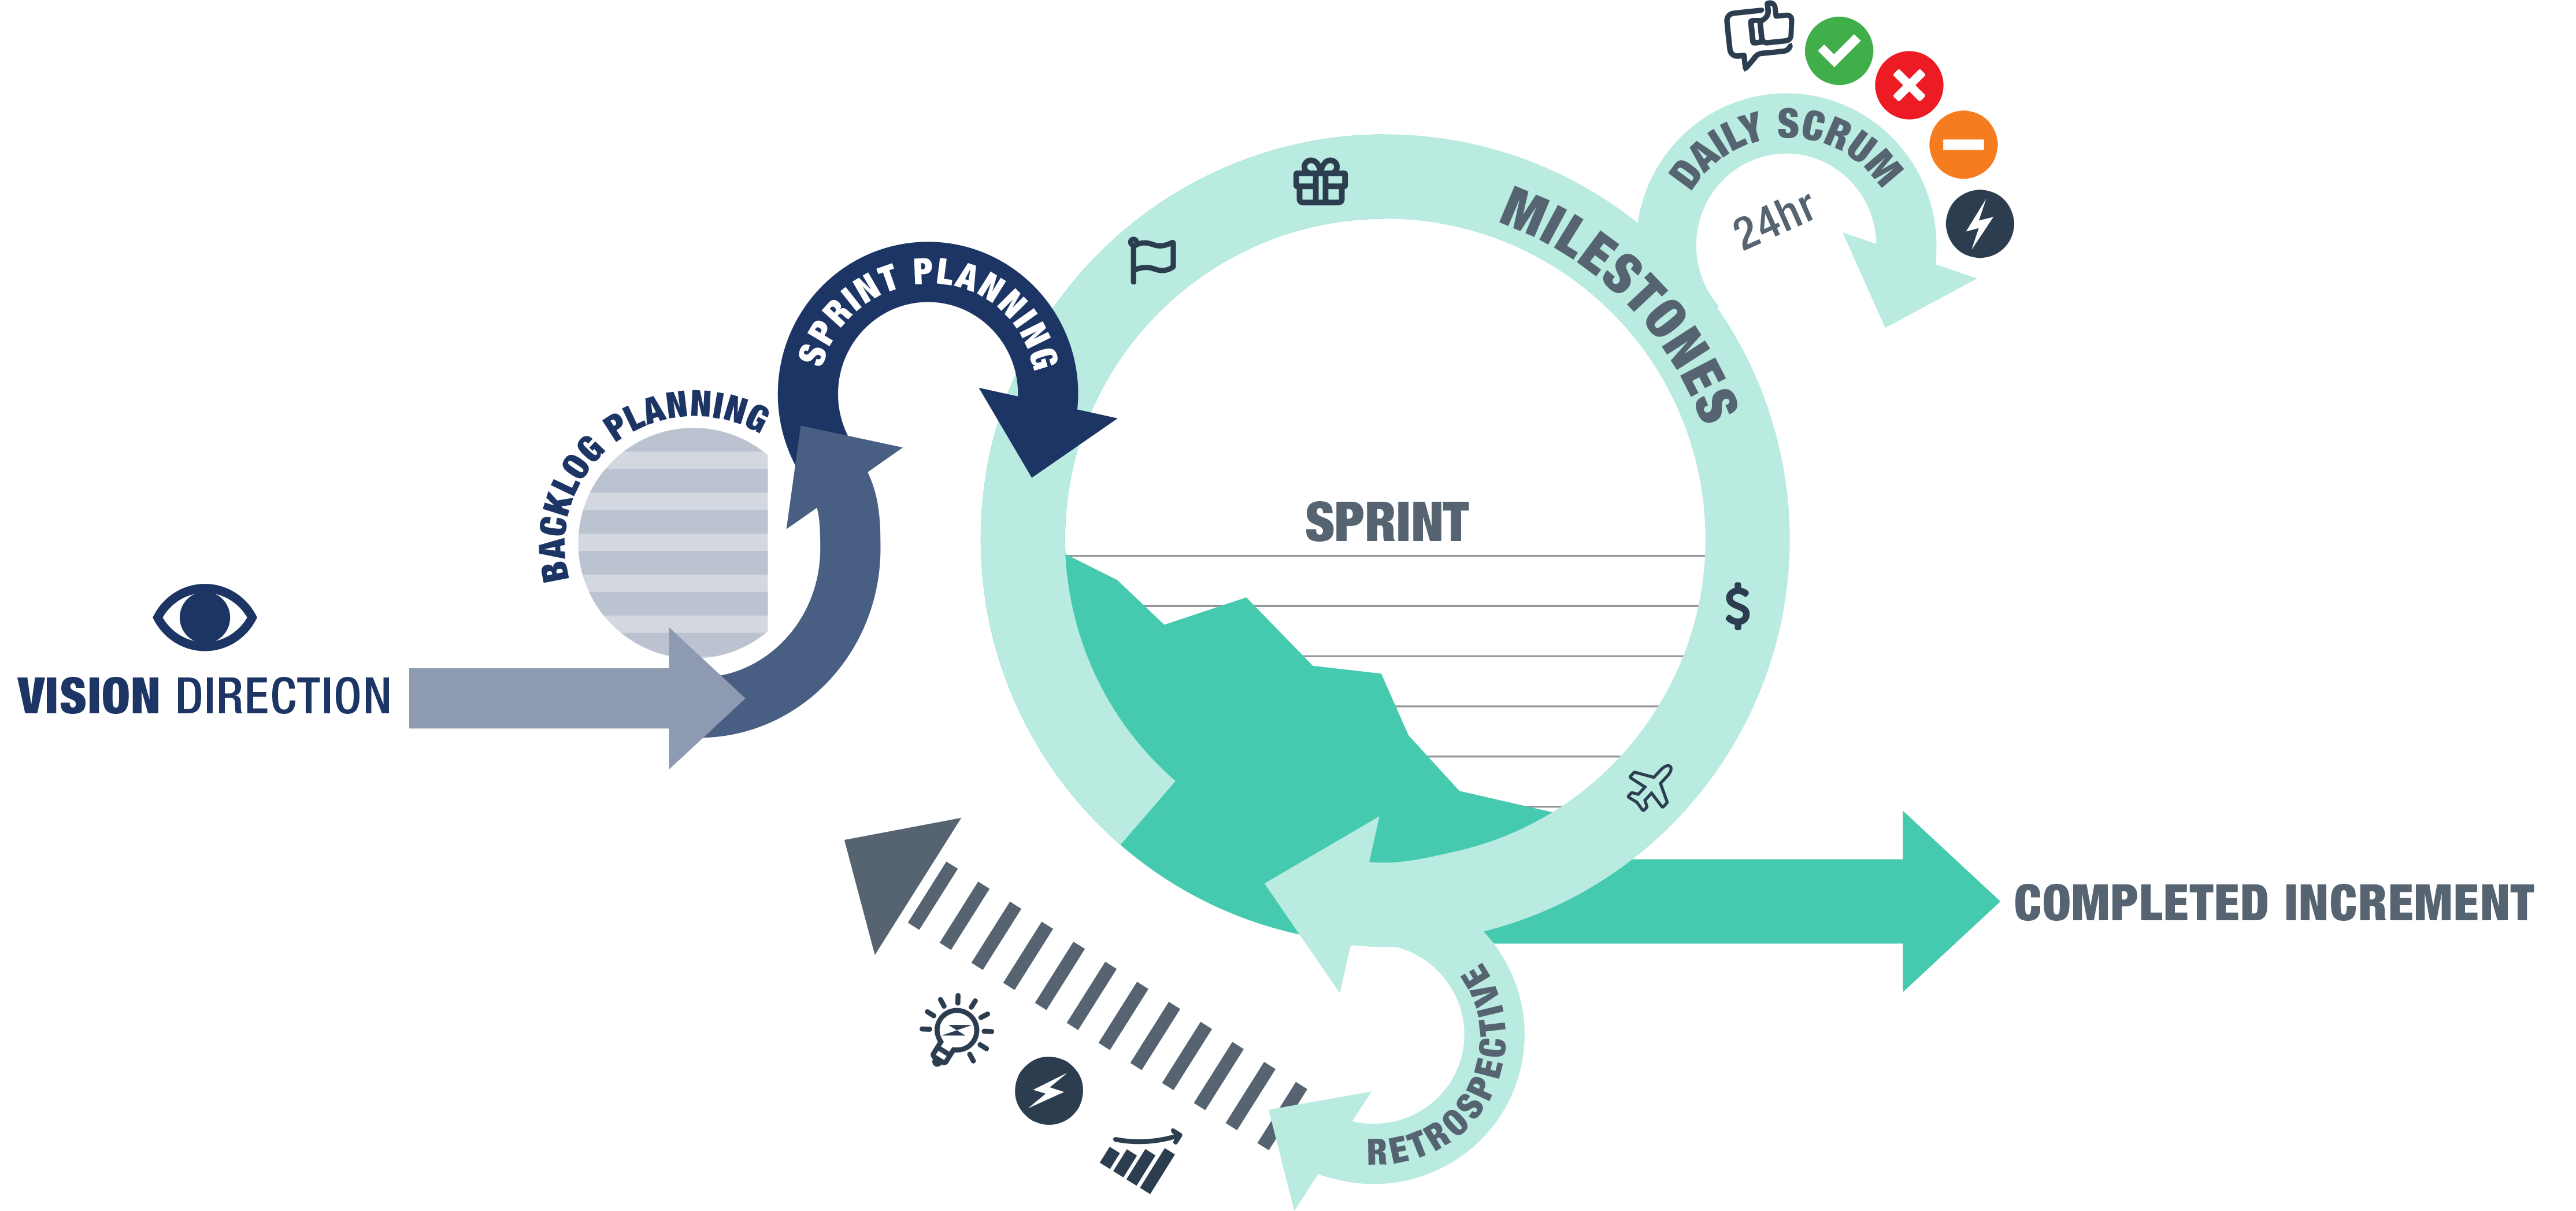
\includegraphics[width=0.8\textwidth]{agile-scrum.png}
      \caption{Scrum Methodology}
    \end{figure}
  \end{frame}

  \begin{frame}{Tools and Technologies}
    \begin{itemize}
      \begin{multicols}{2}
      \item \faNode{} Node.js
      \item Solidity (Smart contract)
      \item \faCodeBranch{} Github Actions (CI/CD)
      \item \faReact{} Next.js (React.js framework)
      \item Hardhat (Solidity framework)
      \item \faDocker{} Docker (Deployment)
      \item Ethers (Library)
      \item Infura (IPFS gateway)
      \end{multicols}
    \end{itemize}
  \end{frame}

  \section{Diagrams}

  \begin{frame}{dApp Architecture}
    \begin{figure}
      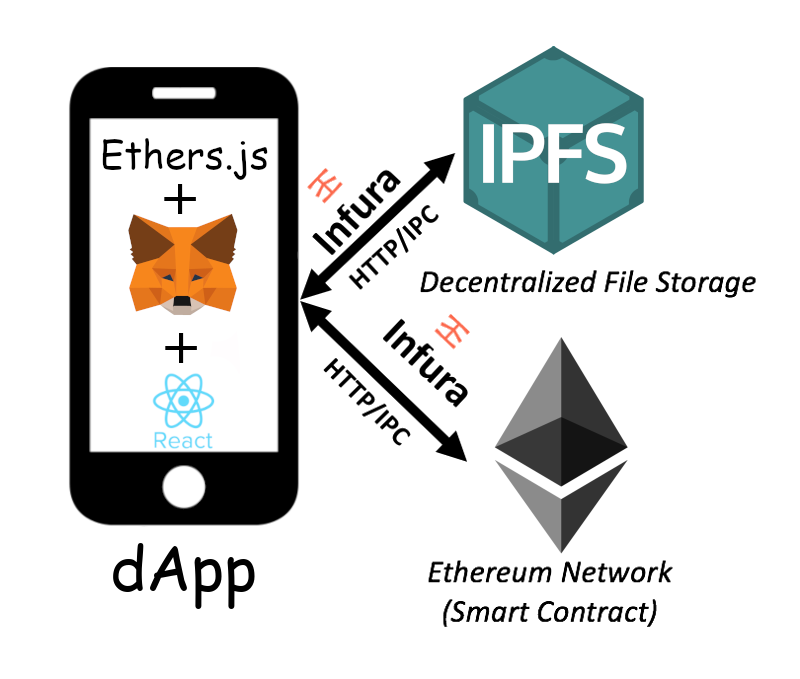
\includegraphics[width=0.53\textwidth]{dapp-arch.png}
      \caption{dApp Architecture}
    \end{figure}
  \end{frame}

  \begin{frame}{Project Diagram}
    \begin{figure}
      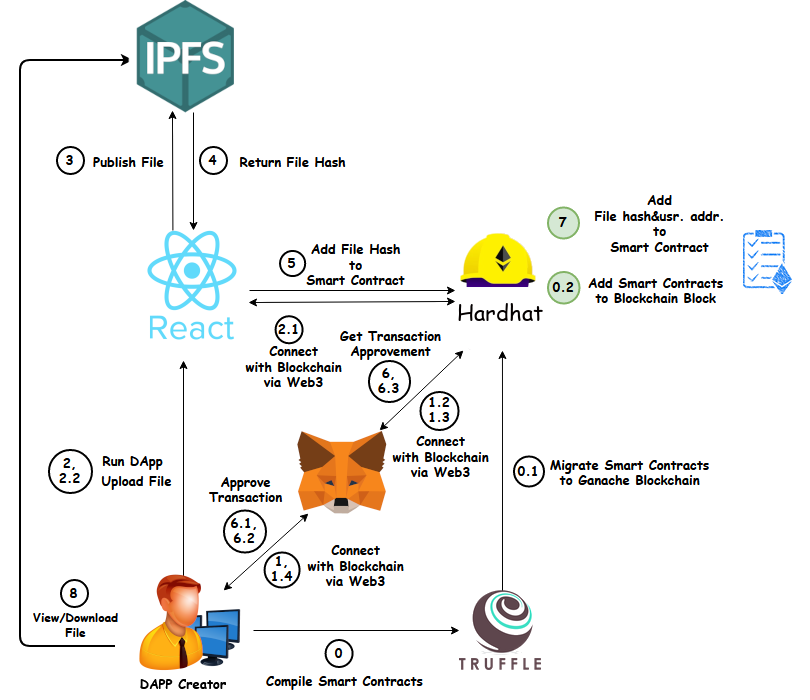
\includegraphics[width=0.53\textwidth]{project-diagram.png}
      \caption{Project Diagram}
    \end{figure}
  \end{frame}

	\begin{frame}[standout]
		Thanks!
	\end{frame}

	\begin{frame}[allowframebreaks]{References}
    \nocite{*}
    \bibliography{biblio}
		\bibliographystyle{unsrt}
	\end{frame}

\end{document}
